\section{YOLO11-DLA}
\label{sec:method}
\begin{figure*}[t]
\centering
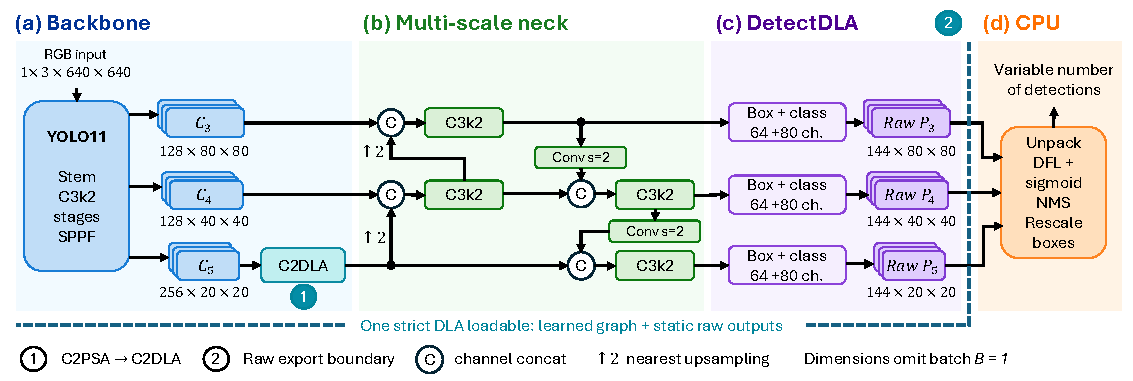
\includegraphics[width=0.95\textwidth]{figures/architecture_overview.pdf}
\caption{\textbf{YOLO11-DLA architecture.} Backbone scales feed the neck and box/class
 towers at strides 8, 16, and 32. Markers 1 and 2 identify C2DLA and the raw-output
 boundary. The learned graph forms one DLA loadable; unpacking and post-processing
 remain on CPU. Preprocessing and input packing precede the graph.}
\label{fig:boundary}
\end{figure*}

\subsection{Design Objective and Scope}
This work treats learned-graph placement as a design constraint for embedded
robotic perception. Let $G$ denote the learned graph obtained by adapting the
reference YOLO11 graph. The design goal is to obtain a useful detector whose
complete learned computation can be assigned to the tested DLA configuration:
\begin{equation}
 \operatorname{Build}_{\mathrm{DLA}}(G;\theta,\mathrm{fallback}=0)
 = E, \qquad N_{\mathrm{GPU}}(E)=0,
 \label{eq:accept}
\end{equation}
where $\theta$ fixes the target, compiler version, precision, shapes, and
I/O formats, $E$ is the serialized engine, and $N_{\mathrm{GPU}}$ counts
GPU-assigned learned layers after optimization. For each evaluated strict
engine, one DLA loadable is also required. These are deployment criteria, not training-loss
terms; accuracy and application performance are evaluated after this gate.

The convolutional stem, C3k2 stages, SPPF module, feature-pyramid connections,
and detection towers of YOLO11n are retained (Fig.~\ref{fig:boundary}). Two module substitutions define
the adaptation:
\begin{equation}
 \mathrm{C2PSA}\longrightarrow\mathrm{C2DLA},\qquad
 \mathrm{Detect}\longrightarrow\mathrm{DetectDLA}.
 \label{eq:substitutions}
\end{equation}
The first substitution changes an accelerator-incompatible learned computation;
the second defines a static accelerator boundary while preserving the ordinary
training path. Together they retain the surrounding YOLO11 backbone, neck,
and detection towers. The adapted GPU engine provides a same-model placement
control; comparisons with stock YOLO11n additionally include architectural and
training differences and use different prediction interfaces.

\subsection{C2DLA: Channel Mixing with Local Context}
\label{sec:c2dla}
\begin{figure*}[t]
\centering
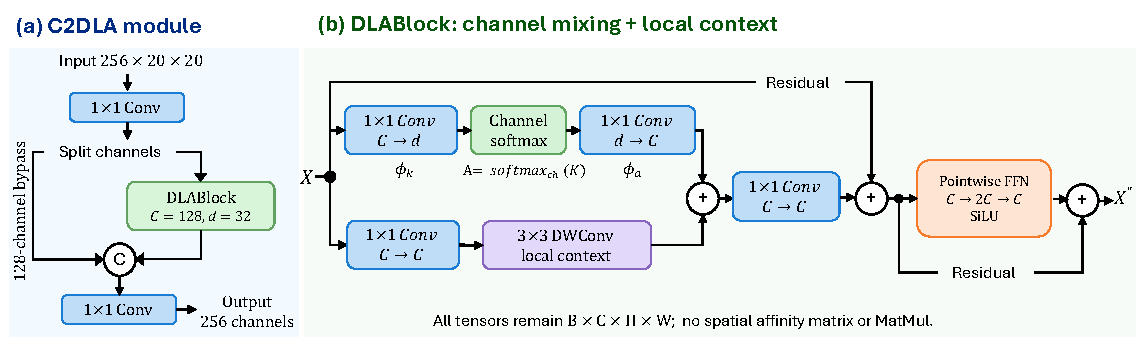
\includegraphics[width=0.90\textwidth]{figures/c2dla_detail.pdf}
\caption{\textbf{C2DLA module and operators.} (a) Nano-model split--process--merge block
 at $20\times20$. (b) Channel softmax and local depthwise convolution replace spatial
 attention, retaining both residual additions and the pointwise FFN.
 C denotes concatenation; $+$ denotes elementwise addition.}
\label{fig:c2dla}
\end{figure*}

C2DLA keeps C2PSA's split--process--merge structure (Fig.~\ref{fig:c2dla}). An initial $1\times1$
projection produces two channel groups; one bypasses the inner block and the
other is processed before concatenation and a final projection. If $X$ is the
processed group with $C$ channels, define
\begin{align}
 K &= \phi_k(X), \qquad V=\phi_v(X), \label{eq:kv}\\
 A_{bkhw} &= \frac{\exp K_{bkhw}}{\sum_{j=1}^{d}\exp K_{bjhw}},
 \label{eq:chansoftmax}\\
 Z &= \phi_o\bigl(\phi_a(A)+\psi_{3\times3}(V)\bigr),
 \label{eq:mix}\\
 X' &= X+Z, \label{eq:res1}\\
 X'' &= X'+\operatorname{FFN}(X'). \label{eq:res2}
\end{align}
Here $d=\max(\lfloor C/4\rfloor,8)$; $\phi_k:C\to d$,
$\phi_v:C\to C$, $\phi_a:d\to C$, and $\phi_o:C\to C$ are
$1\times1$ projections. The operator $\psi$ is a $3\times3$ depthwise
convolution. The FFN expands channels from $C$ to $2C$, applies SiLU, and
projects back to $C$. Batch normalization accompanies the relevant convolution
modules and is folded into them for inference; $\phi_a$ is a bias-free
convolution without batch normalization.

For the nano configuration, the enclosing block receives 256 channels, the
processed group has $C=128$, the bottleneck has $d=32$, and one inner block
operates at the $20\times20$ scale. All operations preserve the four-dimensional
batch--channel--height--width representation. Unlike the original attention,
there is no spatial affinity matrix, matrix multiplication, head transpose,
or normalization over image positions.

This hardware-aware substitute uses input-dependent channel mixing and
local depthwise context while operating on static four-dimensional tensors and
avoiding spatial affinity matrices and MatMul. It does not exchange information
between distant positions. The substitution changes the hypothesis class and
requires empirical accuracy evaluation; it is not algebraically equivalent to
C2PSA, nor is greater representational power claimed.

The key and value projections are separate convolutions. This avoids introducing
a fused-QKV extraction subgraph in the replacement branch. Static channel
splits elsewhere in the retained graph remain present and compile successfully
in the measured configuration. Thus, the implementation does not depend on a
claim that every split or SiLU is unsupported on DLA.

\subsection{DetectDLA: A Static Prediction Boundary}
\label{sec:boundary}
For each pyramid level $\ell\in\{3,4,5\}$, the retained regression and
classification towers produce $R_\ell$ and $S_\ell$. DetectDLA exports
\begin{equation}
 P_\ell=\operatorname{Concat}_{C}(R_\ell,S_\ell)
 \in\mathbb{R}^{B\times(4r+n_c)\times H_\ell\times W_\ell},
 \label{eq:packed}
\end{equation}
with $r=16$ regression bins and $n_c=80$ COCO classes. For batch one and
$640\times640$ images, the outputs are $1\times144\times80\times80$,
$1\times144\times40\times40$, and $1\times144\times20\times20$ at strides
8, 16, and 32. They are named \texttt{pred\_p3}, \texttt{pred\_p4}, and
\texttt{pred\_p5}. Classification values are logits; box channels are
unnormalized distributions, not decoded coordinates.

DetectDLA defines the boundary between a static learned accelerator graph and
host-side detection processing. Export stops before flattening, cross-scale
concatenation, the expectation over the DFL regression distribution, grid
decoding, and
sigmoid; confidence filtering and variable-cardinality NMS remain outside the
engine. During training and ordinary PyTorch inference, DetectDLA invokes the
inherited Detect path, retaining its losses and assignment behavior. The change
concerns deployment partitioning, not a direct-regression or one-to-one
prediction formulation.

The static maps make the execution boundary explicit. Stock YOLO11n's engine
instead emits a decoded $1\times84\times8400$ tensor. At FP16, the adapted
outputs contain 2,419,200 bytes, compared with 1,411,200 bytes for the stock
output, a factor of 1.714. Consequently, lower engine-plus-transfer latency does
not by itself establish a faster end-to-end detector pipeline: the adapted FP16
pipeline transfers more data and performs decoding on the host.


\subsection{Training and Initialization}
The nano model is initialized from pretrained YOLO11n weights. The loader
intersects the source and destination state dictionaries by tensor name and
shape, copies compatible entries, and loads them non-strictly. Unmatched
parameters retain their model initialization. This transfers the compatible
backbone, neck, detection towers, and matching parts of the replacement block
without requiring a correspondence between spatial attention and channel mixing.
All trainable layers are subsequently fine-tuned; the procedure does not
require a separate frozen-backbone stage or a specialized QKV remapping.

The model is fine-tuned on COCO train2017 for 500 epochs, with batch size 32,
$640\times640$ images, seed 0, automatic mixed precision (AMP), and no
user-frozen layers. The model contains 2,615,696 unfused parameters. In the
training implementation used for these experiments,
\texttt{optimizer=auto} selects MuSGD for this training budget, with base
learning rate 0.01, momentum 0.9, and weight decay $5\times10^{-4}$.
The schedule has three warm-up epochs followed by linear decay to 0.01 of
the base learning rate; selected classification-head parameter groups use
a threefold learning-rate multiplier. The recorded group learning rates
are consistent with this configuration.

Training uses HSV perturbation, translation, scaling, horizontal flips, and
mosaic augmentation; mosaic is disabled for the final ten epochs. MixUp and
copy-paste are disabled. These settings describe fine-tuning of the adapted
model from stock weights, not equal-budget retraining of both architectures, so
the comparison evaluates the resulting detectors rather than the substitution
alone.
